\question[15]  Ryan va a colocar un tendedero para ropa en su patio trasero rectangular.
Quiere colgarlo entre dos árboles en el borde de su terreno.
Midió su terreno, e hizo el bosquejo de la figura \ref{fig:des_pitagoras_05}, donde todas las longitudes están en metros:
\begin{figure}[H]
    \begin{center}
        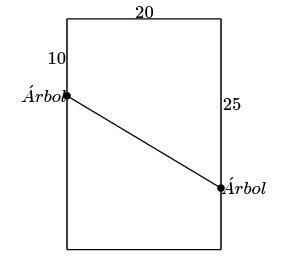
\includegraphics[width=0.3\textwidth]{../images/des_pitagoras_05.png}
    \end{center}
    \caption{}
    \label{fig:des_pitagoras_05}
\end{figure}

\textbf{¿Cuál es la mínima longitud de cuerda que Ryan puede comprar para que se extienda de un árbol al otro?}
